%% This is file `sample-authordraft.tex',
%% generated with the docstrip utility.
%%
%% The original source files were:
%%
%% samples.dtx  (with options: `authordraft')
%% 
%% IMPORTANT NOTICE:
%% 
%% For the copyright see the source file.
%% 
%% Any modified versions of this file must be renamed
%% with new filenames distinct from sample-authordraft.tex.
%% 
%% For distribution of the original source see the terms
%% for copying and modification in the file samples.dtx.
%% 
%% This generated file may be distributed as long as the
%% original source files, as listed above, are part of the
%% same distribution. (The sources need not necessarily be
%% in the same archive or directory.)
%%
%% The first command in your LaTeX source must be the \documentclass command.
\documentclass[sigconf]{acmart}
%% NOTE that a single column version may be required for 
%% submission and peer review. This can be done by changing
%% the \doucmentclass[...]{acmart} in this template to 
%% \documentclass[manuscript,screen,review]{acmart}
%% 
%% To ensure 100% compatibility, please check the white list of
%% approved LaTeX packages to be used with the Master Article Template at
%% https://www.acm.org/publications/taps/whitelist-of-latex-packages 
%% before creating your document. The white list page provides 
%% information on how to submit additional LaTeX packages for 
%% review and adoption.
%% Fonts used in the template cannot be substituted; margin 
%% adjustments are not allowed.
%%
%% \BibTeX command to typeset BibTeX logo in the docs
\AtBeginDocument{%
  \providecommand\BibTeX{{%
    \normalfont B\kern-0.5em{\scshape i\kern-0.25em b}\kern-0.8em\TeX}}}

%% Rights management information.  This information is sent to you
%% when you complete the rights form.  These commands have SAMPLE
%% values in them; it is your responsibility as an author to replace
%% the commands and values with those provided to you when you
%% complete the rights form.


\setcopyright{acmcopyright}
\copyrightyear{2021}
\acmYear{2021}
\acmDOI{}

%% These commands are for a PROCEEDINGS abstract or paper.
\acmConference[Seminar Data Science]{Ulm: Seminar Data-Science}{20/21}{Ulm, Germany}
\acmBooktitle{University Ulm: Seminar Data Science}

%%
%% Submission ID.
%% Use this when submitting an article to a sponsored event. You'll
%% receive a unique submission ID from the organizers
%% of the event, and this ID should be used as the parameter to this command.
%%\acmSubmissionID{123-A56-BU3}

%%
%% The majority of ACM publications use numbered citations and
%% references.  The command \citestyle{authoryear} switches to the
%% "author year" style.
%%
%% If you are preparing content for an event
%% sponsored by ACM SIGGRAPH, you must use the "author year" style of
%% citations and references.
%% Uncommenting
%% the next command will enable that style.
%%\citestyle{acmauthoryear}
\usepackage{tikz}
%%
%% end of the preamble, start of the body of the document source.
\begin{document}

%%
%% The "title" command has an optional parameter,
%% allowing the author to define a "short title" to be used in page headers.
\title{Temporal Graph Embedding}

%%
%% The "author" command and its associated commands are used to define
%% the authors and their affiliations.
%% Of note is the shared affiliation of the first two authors, and the
%% "authornote" and "authornotemark" commands
%% used to denote shared contribution to the research.
\author{Justin Mücke}
\email{justin.muecke@uni-ulm.com}
\affiliation{%
  \institution{University Ulm}
  \streetaddress{Albert-Einstein-Allee}
  \city{Ulm}
  \country{Germany}
  \postcode{89077}
}



%%
%% By default, the full list of authors will be used in the page
%% headers. Often, this list is too long, and will overlap
%% other information printed in the page headers. This command allows
%% the author to define a more concise list
%% of authors' names for this purpose.
\renewcommand{\shortauthors}{Justin Mücke}

%%
%% The abstract is a short summary of the work to be presented in the
%% article.
\begin{abstract}
  
\end{abstract}


%%
%% Keywords. The author(s) should pick words that accurately describe
%% the work being presented. Separate the keywords with commas.
\keywords{Temporal Graph, Embedding}

%% A "teaser" image appears between the author and affiliation
%% information and the body of the document, and typically spans the
%% page.


%%
%% This command processes the author and affiliation and title
%% information and builds the first part of the formatted document.
\maketitle

\section{Introduction}

To start this paper out, let's first create a level playing field for all readers by laying out what exactly a Graph is, 
how it can change over time and what is meant when we talk about embedding.



\subsection{Graphs}
A graph is a mathematical construct which is used in a variety of tasks. It is often used to model relationships between 
entities, thus making it possible to operate on such structures to, for example, analyze them.\\
\begin{figure}[h]
  \begin{center}
    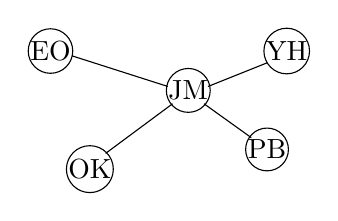
\begin{tikzpicture}
      \draw (0,-0.5) node [circle,inner sep=0pt,draw] {EO};
      \draw (1.75,-1) node [circle,inner sep=0pt,draw] {JM};
      \draw (0.5,-2) node [circle,inner sep=0pt,draw] {OK};
      \draw (3,-0.5) node [circle,inner sep=0pt,draw] {YH};
      \draw (2.75,-1.75) node [circle,inner sep=0pt,draw] {PB};

      \draw (0.27, -0.56) -- (1.49, -0.95);
      \draw (1.55, -1.17) -- (0.7, -1.8);
      \draw (2, -0.95) -- (2.75, -0.65);
      \draw (1.95, -1.17) -- (2.55, -1.6);
    \end{tikzpicture}
\end{center}
\caption{Part of the follower-relationship-graph of personal Instagram account.}
\end{figure}
 Mathematically it is consisting of two sets \(G = (V, E)\), where V consists of all the vertices of the Graph, and E of all the edges, represented through a tuple of two vertices.
 Our graph above would thus look like following: \\
 \( G_i = (\{E,O,Y,P,J\}, \{(J,E),(J,O), (J,P), (J,Y)\}) \).

\subsection{Temporal Graphs}
A temporal graph, on the other hand, is a graph that changes its structure over time. This happens when either one of our sets \((V,E)\) changes. %%Zweiter Satz zu umgs.
Our graph \(G\) is then represented through \(G = \{g_1, g_2, \ldots, g_t\}\) where \(g_i\) is the static graph after time \(i*\Delta t\).
\cite{temporalGraphs}
%TODO Evtl noch erweitern


\subsection{Embedding}
Embedding is a process in which the graph \(G = (V_g, E_g)\) is transformed into a set of vectors \(V\).
These capture the graph topology, vertex-to-vertex relationship as well as other relevant information.
This way, it is more accessible for analyzing the graph and comparing it to others.
Overall we can divide graph embedding techniques into two categories; 
vertex embedding and graph embedding. \\
When using vertex embedding, there has to be one vector \(v\) for each node in \(G\), so that \(|V| = |V_g|\). This is used to make prediction 
on a node level.\\
When using graph embedding, there is one vector representing the whole graph. Most useful is this method to analyze the data on a graph level e.g.
comparing two graph structures with each other.\\
In order to achieve this transformation there are several methods available.

\subsubsection{Word2Vec}
The first method is word2vec which is the foundation for many other methods. 
It takes a text \(T = (w_1, w_2, \ldots, w_n)\) as input and returns a set of vectors\(V\), where \(v_i\) is a distribution describing how likely it is for each word 
to be a direct neighbor to it. The neighbors of a word \(w_c\) are defined as \(\{w_i | i \in (c-\epsilon, c+\epsilon)\}\) where \(\epsilon\) describes a predefined window size.
With this, the whole text it represented solely through vectors, where similar words have similar vectors.
One way to achieve this is to train a neural network to create the distributions. This neural network consists of one input-, one hidden- and one output layer. 
Each word in our text is assigned an ID through a one-hot coded vector, so that each word \(w_i\) can be represented like \((0_1, 0_2, \ldots, 0_{i-1}, 1_i, 0_{i+1}, \ldots 0_n)\).
It then computes how likely it is for each word to be its neighbor and transforms it into a distribution using a softmax-function\cite{softmax}.



\begin{figure}[h]
  \begin{center}
    \scalebox{0.8}{
    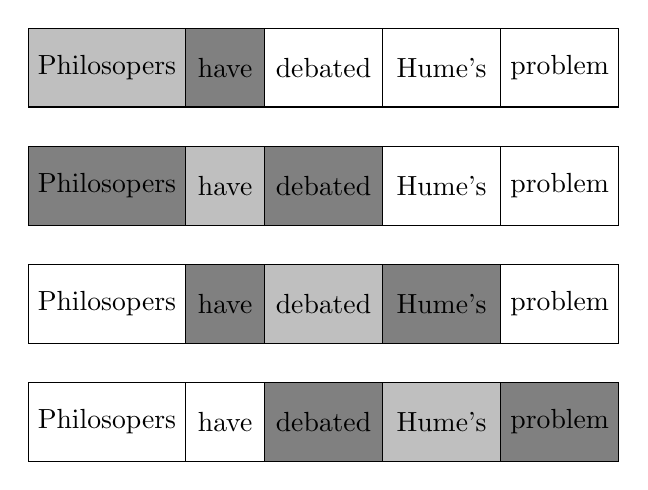
\begin{tikzpicture}
      \draw (0,0) rectangle (2,1) node[pos=.5] {Philosopers};  
      \draw (2,0) rectangle (3,1) node[pos=.5] {have};  
      \draw [fill=gray](3,0) rectangle (4.5,1) node[pos=.5] {debated};  
      \draw [fill=lightgray](4.5,0) rectangle (6,1) node[pos=.5] {Hume's};  
      \draw [fill=gray](6,0) rectangle (7.5,1) node[pos=.5] {problem}; 

      \draw (0,1.5) rectangle (2,2.5) node[pos=.5] {Philosopers};  
      \draw [fill=gray](2,1.5) rectangle (3,2.5) node[pos=.5] {have};  
      \draw [fill=lightgray](3,1.5) rectangle (4.5,2.5) node[pos=.5] {debated};  
      \draw [fill=gray](4.5,1.5) rectangle (6,2.5) node[pos=.5] {Hume's};  
      \draw (6,1.5) rectangle (7.5,2.5) node[pos=.5] {problem}; 

      \draw [fill=gray](0,3) rectangle (2,4) node[pos=.5] {Philosopers};  
      \draw [fill=lightgray](2,3) rectangle (3,4) node[pos=.5] {have};  
      \draw [fill=gray](3,3) rectangle (4.5,4) node[pos=.5] {debated};  
      \draw (4.5,3) rectangle (6,4) node[pos=.5] {Hume's};  
      \draw (6,3) rectangle (7.5,4) node[pos=.5] {problem}; 

      \draw [fill=lightgray](0,4.5) rectangle (2,5.5) node[pos=.5] {Philosopers};  
      \draw [fill=gray](2,4.5) rectangle (3,5.5) node[pos=.5] {have};  
      \draw (3,4.5) rectangle (4.5,5.5) node[pos=.5] {debated};  
      \draw (4.5,4.5) rectangle (6,5.5) node[pos=.5] {Hume's};  
      \draw (6,4.5) rectangle (7.5,5.5) node[pos=.5] {problem}; 

    \end{tikzpicture}}
  \end{center}
  \caption{Light-gray word, with dark-gray neighbor and \(\epsilon = 1\)}
\end{figure}

\subsubsection{DeepWalk}
This method is a continuation of the word2vec approach. 
Overall, the method consists of three steps. First the sampling, which is done using random walks on our graph starting on a selected node.
Hereby, a random walk describes a random succession of nodes of defined length. It is sufficient to perform 32 to 64 random Walks per node.
Those random walks are now of the same form as sentences used in the word2vec method, meaning we can train a similar neural network for predicting
the neighborhood of our nodes.

\subsubsection{Node2Vec}
Here we modify our DeepWalk method. For that purpose we introduce 2 variables \(P\) and \(Q\), where \(Q\) defines how likely it is to go to an unvisited node,
while \(P\) describes how probable it is to revisit a node.

\subsubsection{Structural Deep Network Embedding}
In contrast to the methods used before, SDNE does not use random walks. It aims to preserve local pairwise similarity which characterizes the local structure, and 
as well as the global network structure.
To achieve this, we use two autoencoder neural network. These get an adjacency vector as input and want to construct node adjacency as output.
We then compute the distance between the two outputs and add it to the loss function of the network.
The total loss function is then computed through summation of the distance loss plus the losses of the two encoders.
At the end we remain with a collection of adjacency vectors which describe the graph structure.

\subsubsection{Graph2Vec}
Now we don't want to represent the nodes as vectors, but the whole graph. For that we have once again three steps. 
In the first step we create sub-graphs for each node and encode then once again in a one-hot code. We then use these sub-graphs to train the network used in 
word2vec to maximize the probability that a predicted sup-graph exists in the input graph. The embedding is then the result of the network.
\cite{EmbeddingSummary}
\newpage
\section{Methods}

\subsection{tbGraphEmbed}
Starting paper
\subsection{sub2vec}
Is used as comparison in starting paper -> Look into

\subsection{Comparison}
How do Methods differ -> nodelevel / Graphlevel?

\subsection{Application}
Why do we use Embedding
\subsubsection{Similarity}
Differences Between graphs (exp - googletrends)
\subsubsection{Anomaly}
Where does it differ

\section{Conclusion}

%%
%% The next two lines define the bibliography style to be used, and
%% the bibliography file.

\begin{thebibliography}{1}
\bibitem{temporalGraphs}
George B. Mertzios and Hendrik Molter and Rolf Niedermeier and Viktor Zamaraev and Philipp Zschoche,
\emph{Computing Maximum Matchings in Temporal Graphs},
37th International Symposium on Theoretical Aspects of Computer Science (STACS 2020), 2020
\bibitem{softmax}
Bolin Gao and Lacra Pavel, \emph{On the Properties of the Softmax Function with Application in Game
Theory and Reinforcement Learning}, CoRR, 2017
\bibitem{EmbeddingSummary}
Primož Godec \emph{Graph Embeddings — The Summary}\\
https://towardsdatascience.com/graph-embeddings-the-summary-cc6075aba007
Dec 31, 2018
\bibitem{tdGraphEmbed: Temporal Dynamic Graph-Level Embedding}
Moran Beladev, Lior Rokach, Gilad Katz, Ido Guy, Kira Radinsky, \emph{tdGraphEmbed: Temporal Dynamic Graph-Level Embedding}, {CIKM} '20: The 29th {ACM} International Conference on Information and Knowledge Management, Virtual Event, Ireland, October 19-23, 2020

\end{thebibliography}
%% If your work has an appendix, this is the place to put it.

\end{document}
%%
%% End of file `sample-authordraft.tex'.
